\documentclass[11pt, twoside]{article}
\usepackage{asp2010}

\usepackage{color}
\usepackage{amsfonts}
\usepackage{graphicx}

\resetcounters

\bibliographystyle{asp2010}

\markboth{Scott J. Badenhorst, Sarah Blyth and Michelle M. Kuttel}{Acceleration of automated HI source extraction.}

\begin{document}
 %

\title{Acceleration of automated HI source extraction} 

\author{Scott~J.~Badenhorst, Sarah~Blyth, and Michelle~M.~Kuttel
\affil{Computer Science Department, University of Cape Town, South Africa}}


\begin{abstract}
We aim to enable fast automated extraction of neutral hydrogen (HI)  sources from large survey data sets. 
This requires both handling the large files ($>$5 TB) to be produced by next-generation interferometers and acceleration of  the source extraction algorithm. 
We develop an efficient multithreaded implementation of the A'Trous wavelet reconstruction algorithm, which we evaluate against the serial implementation in the DUCHAMP package.  We also evaluate three memory management libraries (Mmap, Boost and Stxxl) that enable processing of data files too large to fit into main memory, to establish which provides the best performance. 
\end{abstract}




\section{Introduction}

Deep and wide-field surveys of neutral hydrogen (HI) galaxies on the proposed Square Kilometer Array (SKA) will produce 
large data sets that will make manual extraction of sources infeasible.  Automated source extraction is commonly performed with the SExtractor \citep{Bertin1996} and DUCHAMP software \citep{Whiting2012}.  
 The recent addition to DUCHAMP of  noise removal with A'Trous wavelet reconstruction \citep{West2010} improves the reliability of automated source extraction \citep{Popping2012, Whiting2012}.  
However, the method remains computationally expensive and does not scale to large datasets.  

In this work, we attempt to accelerate the A'Trous wavelet reconstruction algorithm through both algorithmic improvements and parallelization of the filter convolution component. 
The wavelet reconstruction algorithm  principally performs filter convolutions of the data. The scattered memory access pattern of this operation, especially in the 3D case, results in numerous cache misses.  Optimisation with separable filtering techniques (common in image filtering) could reduce the algorithmic complexity. 

In addition, we evaluate three memory management libraries to determine if these will allow scaling to very large datasets with minimal penalty.
The maximum possible data set size is typically constrained by the size of the heap, comprising main memory (up to to 32GB) and pre-allocated disk swop space.  The A'Trous algorithm is memory-intensive: a data set of size N requires 5 to 6N of allocated heap memory,, saturating memory for relatively small datasets.
A solution  is to use memory management libraries, such as Mmap\citep{mmap2012},
that simulate contiguous memory swop space, but dynamically allocate space on disk.
Memory management libraries also attempt to amortise slow disk access with read-ahead heuristics to prefault pages into memory in parallel with computation.



\section{Methods}

We used OpenMP to parallelise the  A'Trous wavelet reconstruction, both with and without separable filtering.  Within the DUCHAMP software, filters are built up from 1D components and are hence inherently separable.  Implementation of separable filtering was constrained to the biggest filter in DUCHAMP: the  5x5x5 B3-Spline.
Separable filtering implementations should  improve performance of this filter by 8.3x over its 3D counterpart \citep{Solomon2010}.
For the parallel implementation, the convolution workload is divided at the filter application level: each  thread filters the surrounding data for a particular voxel to compute its new value and stores the result in
a separate data structure to prevent overwrites as the filters overlap.  All  3D filter implementations were validated against  DUCHAMP, for both single and double precision datasets.

The majority of the data sets used for testing comprise high resolution HI observations of nearby galaxies obtained from the THINGS survey \citep{Walter2008}.
In addition, six synthesized observations were generated and populated with white noise to provide additional data points for evaluation, including the three largest data sets. As run-time is dependent on numerous variables ---  data set volume, the number of scales convolved  and the level of smoothing required ---
we compared the average time of  individual components of the wavelet reconstruction algorithm, rather than the total time.  Runs were performed on a quad-core Intel i7-2600 with 8GB RAM.



Three popular memory management libraries were evaluated on Ubuntu 11.04: Mmap, Boost \citep{Gaz2012} and the Stxxl \citep{Dementiev2005}.
MMap is a low level system call for memory mapping, allowing for simple memory management.
Boost is a multi-threaded library for efficient memory mapping that is easier to implement than MMap.
 Stxxl is an out-of-core implementation of the C++ standard template library which facilitates memory management either with memory mapping or standard file IO.
Use of these libraries does not require any alteration to the algorithm  and allows dataset size to reach
the maximum file size defined by the OS and hardware memory addressing scheme (approximately 1TB).
Both Mmap and Boost have an \emph{madvise}  function to indicate how the memory will be accessed.
For a linear access pattern, the OS is requested to aggressively draw pages into memory, while  a random access pattern will only draw in a single page in from disk and will dispose of the page or write back to disk soon after if it is modified.

The three implemented memory management libraries were timed for sequential and random memory access as well as their performance when coupled to the filter convolution process.  This assessment  was repeated for all dataset sizes, reaching a maximum dataset size of 3GB (18GB heap space required). 



 
\section{Results and Discussion}
  
\begin{figure}[ht]
  \centering
  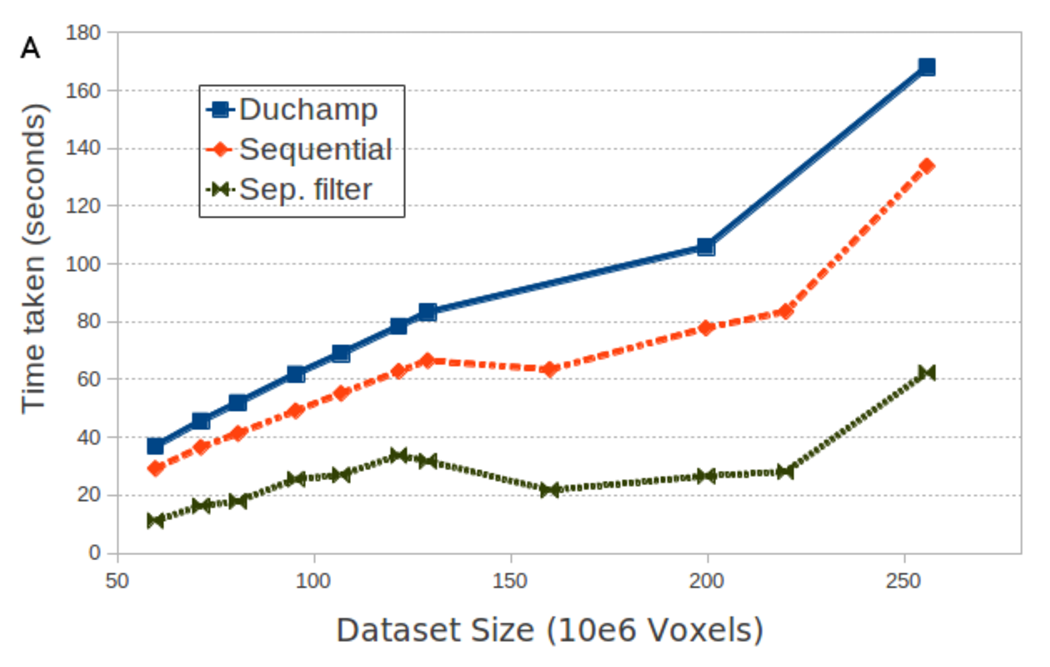
\includegraphics[scale=0.385]{O01_f1}
  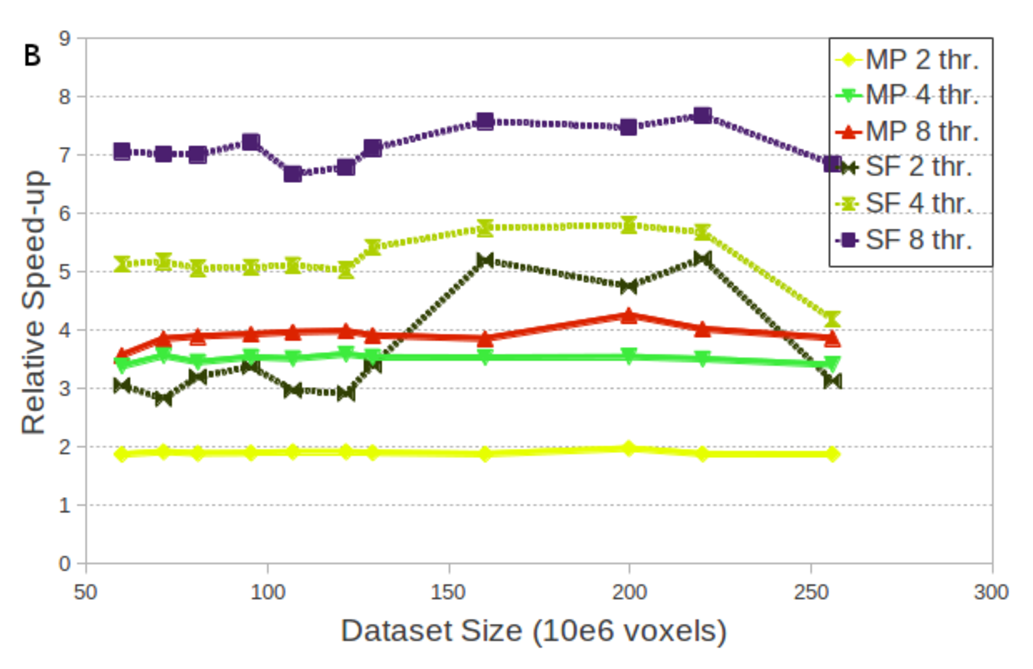
\includegraphics[scale=0.385]{O01_f2}
  \caption{Convolution component of A'Trous Wavelet reconstruction.  (a) Time for a single sequential filter pass (averaged over all scales).  (b) Parallel speeds-ups relative to our own single CPU version achieved for standard 3D (MP) and separable (SF) filtering.} %(c) Time break down for the separable filtering algorithm (sequential). (d) Run times for various memory access patterns coupled with memory management libraries. }
  \label{fig:H2}
\end{figure}



\begin{figure}[ht]
  \centering
  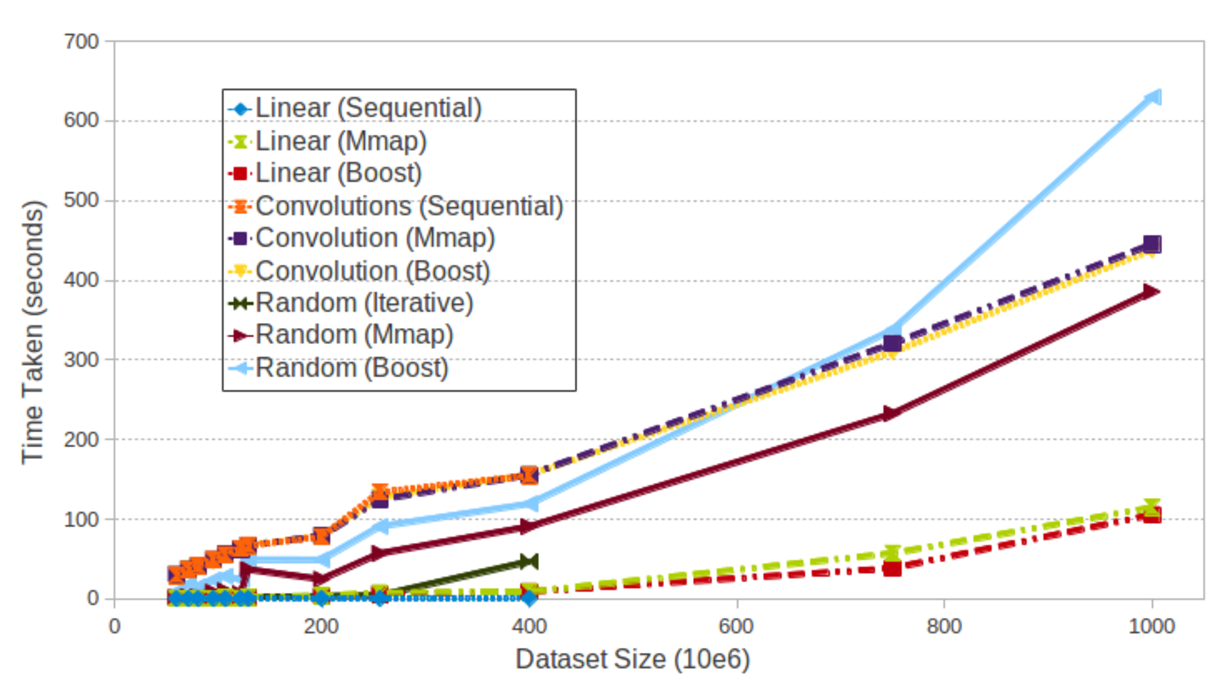
\includegraphics[scale=0.55]{O01_f3}
  \caption{Run-times of the various memory access patterns and  memory management library combinations.} %Shown are random access (quick select method), linear access (the updating of coefficients after a filter pass) and the wavelet reconstruction filter convolution. }
  \label{fig:H3}
\end{figure}


Our sequential implementation outperforms the original DUCHAMP algorithm for all datasets (Fig\ref{fig:H2}A).  It achieves this through removal of an unnecessary  trimming operation (GoodVoxelChecks) for handling padding in non-rectangular observations.  

Separable filtering (green line) achieves a 3x speed-up relative to our 3D filtering implementation  through improved memory access. 
For all sequential implementations, data sets between  120 and 240 million voxels in size run faster than expected. This effect is likely the results of
larger data sets benefiting from caching effects, until  the point that system memory becomes saturated, whereupon paging to disk decreases performance.   %Hmmm,

Multithreading  of the 3D filter convolution  with OpenMP (Fig\ref{fig:H2}B) shows close to ideal speed up across a range of data sets:
on a quad-core CPU, the 2 and 4 thread implementations achieve 1.9x and 3.5x respectively.  The 8-thread implementation shows a 4.2x speedup, a 20\% increase over 4-threads due to  Intel's hyper-threading technology which simulates 8 logical cores. 
Multi-core parallelism in conjunction with separable filtering (Fig\ref{fig:H2}B) shows more significant speed up, with the 4 and 8-thread implementations approaching 5.7x and 7.6x. 


There is large disparity between the Mmap and Boost memory management libraries (Fig\ref{fig:H3}): the Boost library performs  1.3 - 2x slower than Mmap, indicating higher overheads for a random page faults.   The Stxxl library (not shown) was 4-6x slower than Boost and Mmap in our tests.
For small data sets, all libraries are a order of magnitude slower than our sequential implementation (which can only run on smaller data sets due to heap size limits) as overheads are associated with
abstracting the memory heirarchy.
Linear memory access (Fig\ref{fig:H3}) is faster than random access, due to fewer page faults. The read-ahead or pre-faulting is slightly superior (up to 30\% faster) for the Boost library. However, this process is still severely IO bound,  which accounts for the exponential increase in computation time.
The filter convolution component allows for slow disk access to be amortized by pre-faulting pages in parallel with computation. 
The sequential algorithm is  computationally bound, allowing it to scale to extremely large datasets without penalty. The dataset size is only limited by restrictions imposed by the system's addressing scheme. 
However, the slow-down associated with the rest of the algorithm is too severe to justify a memory management port for standard hard disks:
any speed-up obtained through parallelism will likely be IO bound.

\section{Conclusions}

We have demonstrated that multi-core CPU parallelism with OpenMP and reduction in algorithm complexity with separable filtering produces significant speed-ups
for the filter convolution component of the A'Trous wavelet reconstruction algorithm. Additionally, preliminary investigation demonstrated
that standard disk access is to slow for high performance astronomical computing even with the aid of memory management: faster disks or parallel access is required.  Future work will revist memory management coupled with external memory solutions capable of saturating the IO bus.




\begin{thebibliography}{}
\expandafter\ifx\csname natexlab\endcsname\relax\def\natexlab#1{#1}\fi
\expandafter\ifx\csname url\endcsname\relax
  \def\url#1{\texttt{#1}}\fi
\expandafter\ifx\csname urlprefix\endcsname\relax\def\urlprefix{URL }\fi
\providecommand{\eprint}[2][]{\url{#2}}

\bibitem[{Popping et al.(2012)}]{Popping2012}
Popping, A et~al., 2012, PASA, 29, 301

\bibitem[{Whiting(2012)}]{Whiting2012}
Whiting, M.~T. et al., 2012, RAS, 421, 3242-3256

\bibitem[{Dementiev et~al.(2005)}]{Dementiev2005}
Dementiev, R. et al., 2005, Algorithms-ESA 2005, 640-651

\bibitem[{Gaztanaga et~al.(2012)}]{Gaz2012}
Gaztanaga, I., 2012, {Boost.Interprocess}, http://goo.gl/8CJGB, Last accessed 2012 Oct 25

\bibitem[{Mmap.(2012)}]{mmap2012}
Mmap(3)-Linux man page., 2012, http://linux.die.net/man/3/mmap, Last accessed 2012 Oct 25

\bibitem[{Westurland(2010)}] {West2010}
Westerlund, S., 2010, iVEC Internship Report, Available at http://goo.gl/MTqFs. Last accessed 2012 Oct 25


\bibitem[{Dagum.(1998)}]{Dagum1998}
Dagum, L., 1998, {Computational Science \& Engineering}, IEEE 5.1 (1998): 46-55.

\bibitem[{Solomon et~al.(2010)}] {Solomon2010}
Solomon, C. et al, 2010, Fundementals of Digital Image Processing, Wiley-Blackwell


\bibitem[{Bertin(1996)}] {Bertin1996}
Bertin, E., 1996, A\&AS, 117, 393

\bibitem[{Walter et~al.(2008)}] {Walter2008}
Walter, F. et al., 2008, Galaxies in the Local Volume (2008): 97-104.

\end{thebibliography}

\end{document}


